\subsection{Architekturüberblick}\label{subsec:wotarchitecture}

Für das \gls{wot} gibt es verschiedenste Anwendungsfälle. All diese haben Gemeinsamkeiten und Unterschiede, aus denen sich die Anforderungen an eine \glsxtrshort{wot}-Architektur \autocite[vgl.][]{w3c.wot.architecture.20200408} ergeben.

\begin{figure}[H]
  \centering
  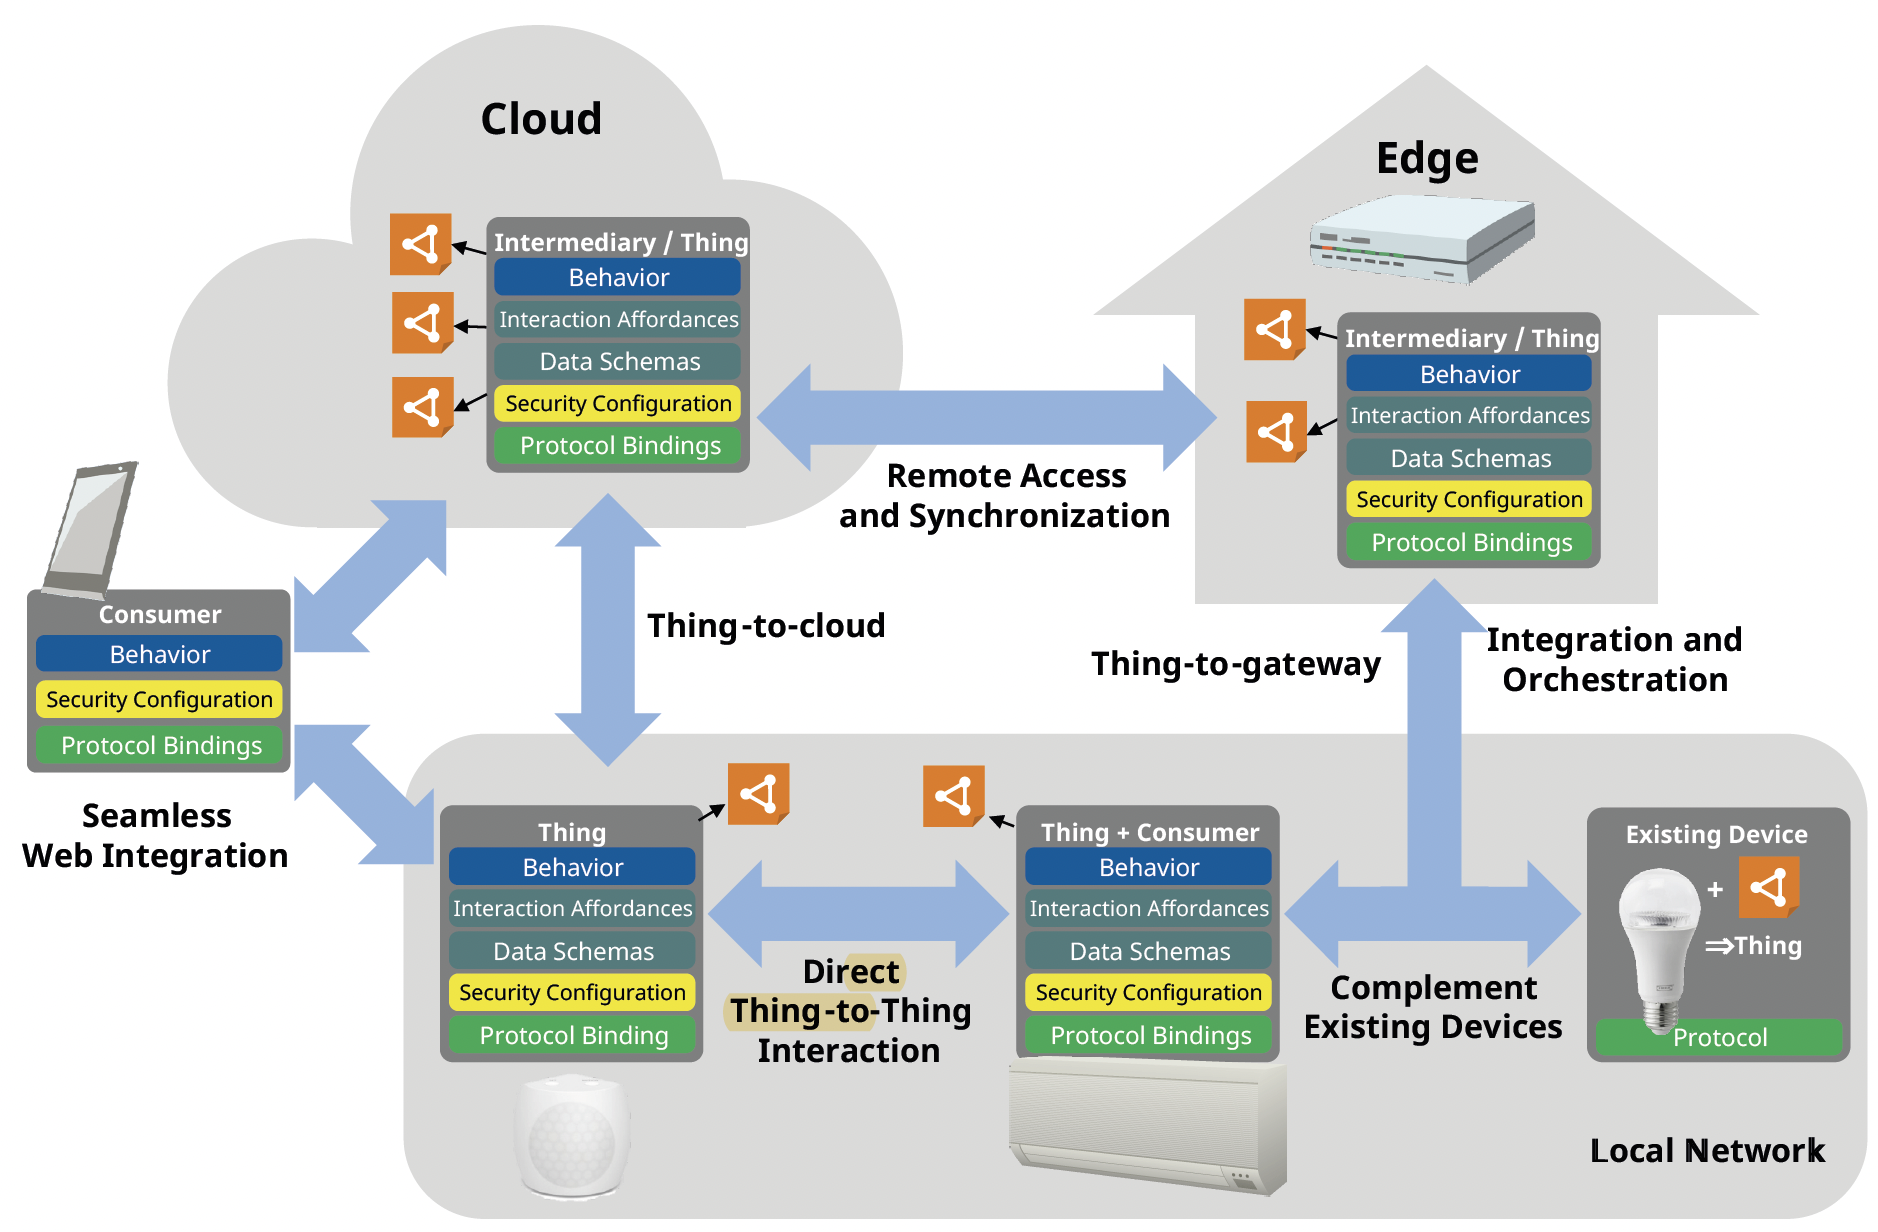
\includegraphics[width=12cm]{abstract-architecture-overview.png}
  \caption{\glsxtrshort{wot}-Architektur}\label{fig:wot_abstract_architecture}
\end{figure}

% Problem Heterogenität

Durch die starke Heterogenität der Anwendungen und Geräte, aber auch der bereits existierenden \glsxtrshort{iot}-Systeme, entsteht eine Vielzahl von Anforderungen. Diese lassen sich häufig in zwei Kategorien einteilen: Positive Anforderungen, die in allen betroffenen Entitäten umgesetzt werden können, oder negative Anforderungen, die nicht in allen betroffenen Entitäten umgesetzt werden können und wodurch die Anforderung aus einer Unabhängigkeit von diesem Teilaspekt besteht. Im Zentrum stehen vier Kernelemente: Flexibilität, Kompatibilität, Skalierbarkeit und Interoperabilität.

% Hardware

Die Architektur muss demnach hardwareunabhängig sein. Auch bestimmte Technologien können nicht vorausgesetzt werden, denn es muss Kompatibilität zu allen vorhandenen Geräten und Systemumgebungen sichergestellt werden. Dadurch fokussiert sich das \gls{wot} des \gls{w3c}[s] auf höhere Systemebenen und somit vor allem die Kommunikationsebene.

% Web Thing

Auf dieser Basis wird die Architektur eines \gls{wt}[s] in verschiedene Bereiche unterteilt. Neben dem eigentlichen \emph{Verhalten} sind das \emph{Interaktionsaffordanzen}, die dazugehörigen \emph{Datenschemata}, die \emph{Sicherheitskonfiguration} und \emph{Protokollbindungen}. Dabei sind die Protokollbindungen die Definition, wie konkret Interaktionen durchgeführt werden können, während die Affordanzen nur beschreiben, was möglich ist, unabhängig von Protokollen oder Datenkodierung. Das \emph{Interaktionsmodell} beschreibt dabei neben Navigation drei weitere Typen von Interaktionsaffordanzen:

\begin{itemize}
  \item \emph{Eigenschaften} bilden den Zustand eines \gls{thing}[s] ab.
  \item Mittels \emph{Aktionen} kann der Zustand eines \gls{thing}[s] oder eine Funktion auf diesem geändert bzw.\ aufgerufen werden. % TODO: Aktionen
  \item \emph{Ereignisse} finden bei Zustandsänderungen statt und können Daten asynchron an \gls{consumer} senden.
\end{itemize}

Dabei werden die einzelnen Interaktionsschnittstellen durch Verknüpfungen in Form von \gls{uri}[s] und optionale Zusatzbeschreibungen maschinenlesbar definiert.

\begin{figure}[H]
  \centering
  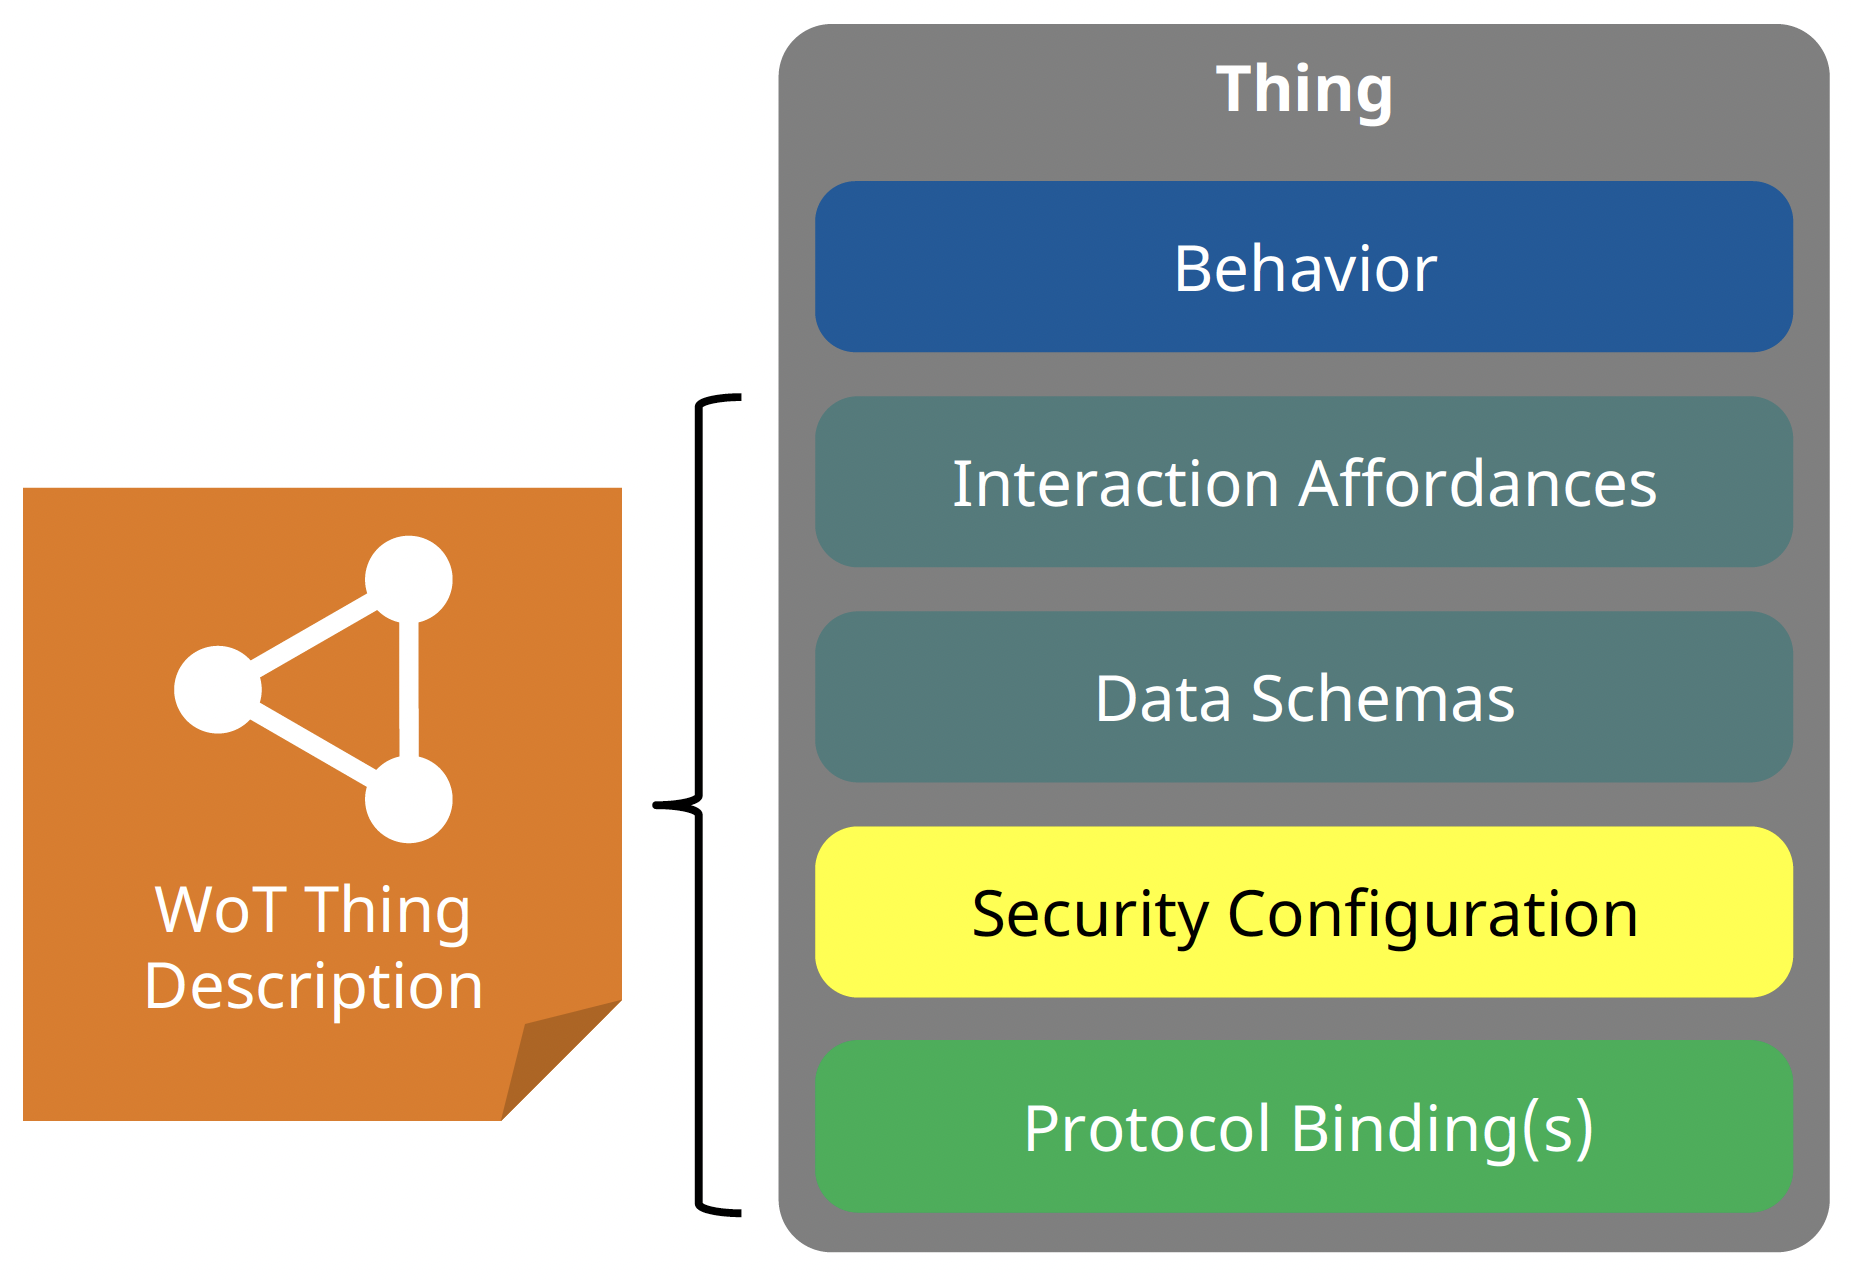
\includegraphics[width=8cm]{thing-architecture.png}
  \caption{\gls{thing}-Architektur}\label{fig:td_thing_architecture}
\end{figure}

% Thing-Beschreibung

Jedes \gls{thing} (oder dessen \gls{intermediary}) muss diese Funktionalitäten und Metadaten über sich bereitstellen können. Dazu gehören die bereits erwähnten Interaktionsaffordanzen, Datenschemata, die Sicherheitskonfiguration und die Protokollbindungen, neben dem Namen oder der Version des \gls{thing}[s] aber nicht zuletzt auch verwandte \glspl{thing}. Diese Eigenschaften sollen sowohl menschenlesbar als auch maschinenlesbar sein, semantisch annotiert werden sowie, falls zutreffend, Internationalisierung unterstützen können. Die Beschreibung dieser Eigenschaften wird \gls{td} genannt. Die \gls{td} wird als \gls{json} übermittelt und dient als Einstiegspunkt für ein \gls{thing}.

Im Idealfall wird eine \gls{td} direkt auf dem jeweiligen \gls{thing} erstellt und bereitgestellt. Domänenspezifisches Vokabular wird dabei zwar nicht durch die \glsxtrshort{wot}-Spezifikationen des \gls{w3c} abgedeckt, da die \gls{td} aber \gls{jsonld} implementiert, kann beliebiges Vokabular als Kontext eingebunden werden. Eine genauere Beschreibung der \glsfmtlong{td} ist in \autoref{subsec:wottd} zu finden.

% Protokolle

\Glspl{wt} müssen verschiedene Protokolle unterstützen können. Dazu zählen nicht nur Internetprotokolle, sondern auch Protokolle, die im \gls{lan} genutzt werden. Außerdem sollten auch Kombinationen von Protokollen genutzt werden können. So soll grundsätzlich mit \glsxtrshort{rest}-\glsxtrshortpl{api} gearbeitet werden, jedoch soll auch der Datenaustausch mit dem \gls{pubsub}-Muster möglich sein.

% Discovery

Damit mit einem \gls{wt} -- also der Repräsentation eines \gls{thing}[s] im Web -- interagiert werden kann, muss ein \gls{consumer} aber von diesem wissen. Dafür muss nach dem \gls{wt} gesucht werden können. Diese Suche muss syntaktisch (Attribute, …) und semantisch (Funktionalitäten auf Basis eines einheitlichen Vokabulars) über verschiedene Formate möglich sein. Es kann hilfreich sein, für die Erkundung ein Verzeichnis zu nutzen, bei dem sich die einzelnen \glspl{wt} automatisiert oder manuell registrieren können und welches darauf basierende Suchanfragen bearbeiten kann. (Siehe dazu auch \autoref{subsec:wotdiscovery}.)

% Sicherheit

Die \gls{td} umfasst auch Angaben zur Sicherheit nach außen. Dazu gehören z.\,B.\ Authentifizierungsmethoden wie Basic oder OAuth2.0. Grundsätzlich sollten (laut der Spezifikation) \gls{td}[s] nur autorisierten Personen zugänglich gemacht werden, da die enthaltenen Metadaten potenziell sensible Informationen beinhalten können. Trotzdem -- oder gerade deswegen -- sollten die Personen, die \gls{td}[s] erstellen oder verwalten, darauf achten, dass nur öffentliche Sicherheitsinformationen -- wie die jeweilige Authentifizierungsmethode -- in einer \gls{td} vorkommen.

% Barrierefreiheit

Barrierefreiheit ist im Rahmen der Spezifikationen kein Thema, da es um die Kommunikation zwischen Anwendungen und Geräten geht und Personen nicht direkt auf das \gls{wot} zugreifen. Allerdings gilt es zu bedenken, dass mit entsprechenden Annotationen möglicherweise Code oder ganze Interfaces generiert werden könnten, sodass die Integration von Barrierefreiheit durchaus auch Auswirkungen auf andere Bereiche hätte.

Weitere Anforderungen, die jedoch nicht zur Thematik der Service Discovery beitragen, können in \citetitle{w3c.wot.architecture.20200408} \autocite{w3c.wot.architecture.20200408} nachgelesen werden.
